\UseRawInputEncoding
\documentclass[conference]{IEEEtran}
\IEEEoverridecommandlockouts


\usepackage[utf8]{inputenc}  
\usepackage[T1]{fontenc}
\usepackage[spanish,es-tabla,es-nodecimaldot,es-noshorthands]{babel}     
\usepackage{textcomp}        
\usepackage{amsmath,amssymb,amsfonts}
\usepackage{siunitx}                
\DeclareSIUnit\dbi{dBi}
\usepackage{graphicx}           
\usepackage{float}                 
\usepackage{placeins}     
\usepackage{url}
\usepackage[hidelinks]{hyperref}           
\usepackage{cite}             
\usepackage{booktabs}
\usepackage{caption}             
\captionsetup{labelfont=bf, textfont=normalfont} 
\usepackage{listings}                
\usepackage{listingsutf8}             
\usepackage{xcolor}               
\definecolor{codebg}{RGB}{248,248,248}
\definecolor{codeframe}{RGB}{220,220,220}
\definecolor{codekw}{RGB}{0,92,197}
\definecolor{codestr}{RGB}{163,21,21}
\definecolor{codecmt}{RGB}{0,128,0}
% Creación del estilo "bonito" para Python / bloques de código de antena
\lstdefinestyle{bonito}{
    language=Python,
    backgroundcolor=\color{codebg},
    basicstyle=\ttfamily\small,
    keywordstyle=\color{codekw}\bfseries,
    stringstyle=\color{codestr},
    commentstyle=\color{codecmt}\itshape,
    numberstyle=\tiny\color{gray},
    numbers=left,
    stepnumber=1,
    frame=single,
    rulecolor=\color{codeframe},
    frameround=tttt,
    framesep=6pt,
    tabsize=2,
    showstringspaces=false,
    breaklines=true,
    upquote=true,
    % Configuración para evitar desbordamientos a la izquierda
    xleftmargin=2em,
    framexleftmargin=2em,
    numbersep=8pt
}

\raggedbottom                
\usepackage{titlesec}
\titlespacing*{\section}{0pt}{1.2ex plus .3ex minus .2ex}{0.8ex}
\titlespacing*{\subsection}{0pt}{1.0ex plus .3ex minus .2ex}{0.6ex}
\titlespacing*{\subsubsection}{0pt}{0.8ex plus .2ex minus .2ex}{0.5ex}

\setlength{\parskip}{0pt}           

\usepackage{enumitem}
\setlist{nosep}                     

\setlength{\abovecaptionskip}{4pt}
\setlength{\belowcaptionskip}{0pt}
\setlength{\textfloatsep}{10pt plus 1pt minus 2pt}
\setlength{\floatsep}{8pt plus 1pt minus 2pt}
\setlength{\intextsep}{8pt plus 1pt minus 2pt}
\renewcommand{\topfraction}{0.9}
\renewcommand{\bottomfraction}{0.8}
\renewcommand{\textfraction}{0.1}
\renewcommand{\floatpagefraction}{0.8}


\def\BibTeX{{\rm B\kern-.05em{\sc i\kern-.025em b}\kern-.08em
    T\kern-.1667em\lower.7ex\hbox{E}\kern-.125emX}}
\sisetup{output-decimal-marker={,}}
\graphicspath{{Figuras/}}
\begin{document}
%%%%%%%%%%%%%%%%%%%%%%%%%%%%%%%%%%%%%%%%%%%%%%%%%%%%%%%%%%%%%%%%%%%%%%%%%%%
\title{Enlace BPSK interior con multitrayectoria: diseño Tx--canal--Rx, receptor de filtro acoplado y caracterización BER vs. $E_b/N_0$ en GNU Radio\\
\large Proyecto Integrador de Comunicaciones II (27145) -- Escenario S3 -- Grupo 5}
\author{\IEEEauthorblockN{Elkin Largo}
\IEEEauthorblockA{\textit{Universidad Industrial de Santander} \\
Bucaramanga, Colombia \\
Código: 2182334 \\
Email: elkin2182334@correo.uis.edu.co}
\and
\IEEEauthorblockN{Stiven Muñoz}
\IEEEauthorblockA{\textit{Universidad Industrial de Santander} \\
Bucaramanga, Colombia \\
Código: 2224110 \\
Email: stiven2224110@correo.uis.edu.co}
\and
\IEEEauthorblockN{Minuk Lee}
\IEEEauthorblockA{\textit{Universidad Industrial de Santander} \\
Bucaramanga, Colombia \\
Email: minuk2220408@correo.uis.edu.co}
}
%%%%%%%%%%%%%%%%%%%%%%%%%%%%%%%%%%%%%%%%%%%%%%%%%%%%%%%%%%%%%%%%%%%%%%%%%%%%
\maketitle

\begin{abstract}
This report presents the design and simulation of a BPSK link for an indoor sensor in a warehouse (scenario S3, multipath). The transmitter keeps the course reference parameters ($R_s=32$~kBd, $R_b=32$~kb/s, $Sps=8$, $f_s=256$~kS/s, rectangular pulse). The channel is a direct path plus one echo with complex gain $\alpha$ and delay $\tau=T_s$, followed by AWGN. A receiver was designed with a rectangular matched filter, eye diagram, one-in-eight sampling at the eye maximum, and a zero-threshold decision. Four tests ($|\alpha|=0$; 0.2; 0.5; 0.8) were simulated in GNU Radio and verified on GNU Radio 3.10.12 (Windows) and 3.10.9 (Linux). The echo splits each BPSK point into $\pm1\pm\alpha$, reduces the vertical eye opening as $2(1-|\alpha|)$ and imprints the comb response $|1+\alpha e^{-j2\pi fT_s}|^2$ on the PSD. With the Phase-4 BER instrument (two template bugs corrected), the measured BER matches BPSK theory within 0.05~dB at $10^{-3}$. The echo penalty at BER $=10^{-3}$ is 1.4~dB for $|\alpha|=0.2$ and 6.3~dB for $|\alpha|=0.5$; with $|\alpha|=0.8$ the target is not reached below 14~dB. Hardware (HackRF) flowgraphs were prepared but not tested on hardware.
\end{abstract}

\begin{IEEEkeywords}
BPSK, multitrayectoria, interferencia intersimbólica, filtro acoplado, diagrama de ojo, BER, $E_b/N_0$, GNU Radio, SDR.
\end{IEEEkeywords}

{\raggedright\small
\textit{Repositorio:} \url{https://github.com/stivenmunoz0133-spec/ComunicacionesII_Grupo5}\par}

\section{Introducción}
En una bodega con estanterías metálicas, paneles y muros de concreto, la señal de un nodo sensor no llega al receptor por un único camino: a la componente directa se suman réplicas reflejadas, atenuadas y retardadas. Las mediciones clásicas de canales interiores describen este fenómeno como llegadas en grupos con dispersión de retardo eficaz de decenas a cientos de nanosegundos \cite{saleh1987,hashemi1993}; en plantas industriales se han medido valores entre 30 y 300~ns, influidos por el inventario y los materiales de construcción \cite{rappaport1989}. Cuando el retardo de la réplica es comparable con la duración del símbolo, el eco se mezcla con el símbolo siguiente y aparece interferencia intersimbólica (ISI); en frecuencia, el canal deja de ser plano y produce desvanecimiento selectivo \cite{proakis2008,rappaport2002}.

El Grupo~5 eligió el escenario S3 de la guía del curso \cite{guia1}: un sensor transmite variables de baja velocidad (estado, temperatura, vibración) hacia una estación de supervisión dentro de una bodega, y la reflexión dominante deforma los símbolos. El objetivo es aislar ese efecto, sin otras fuentes de ISI, para observarlo y medirlo de forma controlada. Este documento presenta el escenario y la decisión de diseño (Sección~III), la arquitectura implementada en GNU Radio, que incluye el receptor exigido en la Guía~2 \cite{guia2}, las cuatro pruebas de perturbación y la caracterización BER de la Fase~4 \cite{guia4} (Sección~IV), y cierra con las conclusiones.

\textbf{Ajuste a la ficha de decisión.} En la ficha ``Decisión Técnica Ciega'' del grupo, el escenario (S3), la perturbación (camino directo + eco), la variable (ganancia compleja del eco) y la justificación escrita corresponden a multitrayectoria. Sin embargo, quedaron marcados el problema P1 y la hipótesis H1, que corresponden a perturbaciones impulsivas. Para que el informe sea coherente se adoptó explícitamente la hipótesis equivalente para multitrayectoria: \emph{al aumentar $|\alpha|$, la constelación recuperada se desdobla, el ojo se cierra en proporción $1-|\alpha|$ y la BER crece para un mismo $E_b/N_0$}.

\section{Objetivos y alcance}

\textbf{Objetivo general:} diseñar, simular y evaluar un enlace BPSK Tx--canal--Rx para un sensor en una bodega con multitrayectoria, cuantificando la degradación producida por un eco de ganancia variable.

\textbf{Objetivos específicos:}
\begin{enumerate}
    \item Configurar el transmisor con parámetros coherentes ($k$, $R_s$, $R_b$, $Sps$, $f_s$, ancho de banda) a partir del archivo base del curso.
    \item Modelar el canal como camino directo más un eco $\alpha\,s(t-\tau)$ con AWGN y diseñar un receptor de filtro acoplado, muestreo y decisión.
    \item Comparar una prueba de referencia con tres niveles de eco (suave, medio y fuerte) mediante PSD, señal temporal, constelación y diagrama de ojo.
    \item Integrar el instrumento BER vs.\ $E_b/N_0$ de la Fase~4, validar la alineación Tx/Rx y contrastar con la teoría.
\end{enumerate}

\textbf{Alcance:} un solo eco con retardo fijo $\tau=T_s$ y fase $0^\circ$ (caso más desfavorable en fase), BPSK con pulso rectangular, sincronización ideal en simulación y AWGN de referencia \texttt{noise\_amp}$=0{,}10$. La medición BER se realizó en simulación, sustituyendo el enlace SDR por el canal simulado. Las copias para HackRF One (Fase~3) se compilaron y su cadena de sincronización se verificó en simulación, pero no se probaron con hardware.

\section{Metodología}

\subsection{Escenario y modelo físico}
La Figura~\ref{fig:escenario} ubica el nodo sensor (Tx) y la estación de supervisión (Rx) en una bodega de unos $40\times24$~m. El camino directo tiene línea de vista; el eco modelado proviene de la cara metálica de una estantería y llega con trayectoria más larga $d_1>d_0$, ganancia compleja $\alpha=|\alpha|e^{j\varphi}$ y retardo $\tau=(d_1-d_0)/c$. Existen otras reflexiones (estantería~4), que se dejan fuera del modelo para aislar un solo mecanismo. El modelo de canal en banda base es
\begin{equation}
    r(t)=s(t)+\alpha\,s(t-\tau)+w(t), \qquad h(t)=\delta(t)+\alpha\,\delta(t-\tau),
    \label{eq:canal}
\end{equation}
cuya respuesta en frecuencia es $|H(f)|^2=|1+\alpha e^{-j2\pi f\tau}|^2$, con máximos $(1+|\alpha|)^2$ y mínimos $(1-|\alpha|)^2$ separados $1/\tau$ en frecuencia.

\textbf{Normalización del retardo.} Con los parámetros del curso, $T_s=1/R_s=31{,}25~\mu$s, lo que equivale a una diferencia de trayectorias de $cT_s\approx9{,}4$~km. En una bodega real ($\tau\sim$100~ns) se cumpliría $\tau/T_s\approx3\times10^{-3}$ y el canal sería prácticamente plano a 32~kBd. Por ello el retardo se fijó en $\tau=T_s$ (8 muestras), un modelo normalizado que reproduce la situación $\tau/T_s=1$. Esa situación se presentaría en la misma bodega si el enlace operara a decenas de MBd ($R_s\approx1/\tau=10$~MBd), sin modificar los parámetros de referencia exigidos por la guía \cite{guia1}.

\begin{figure*}[!t]
\centering
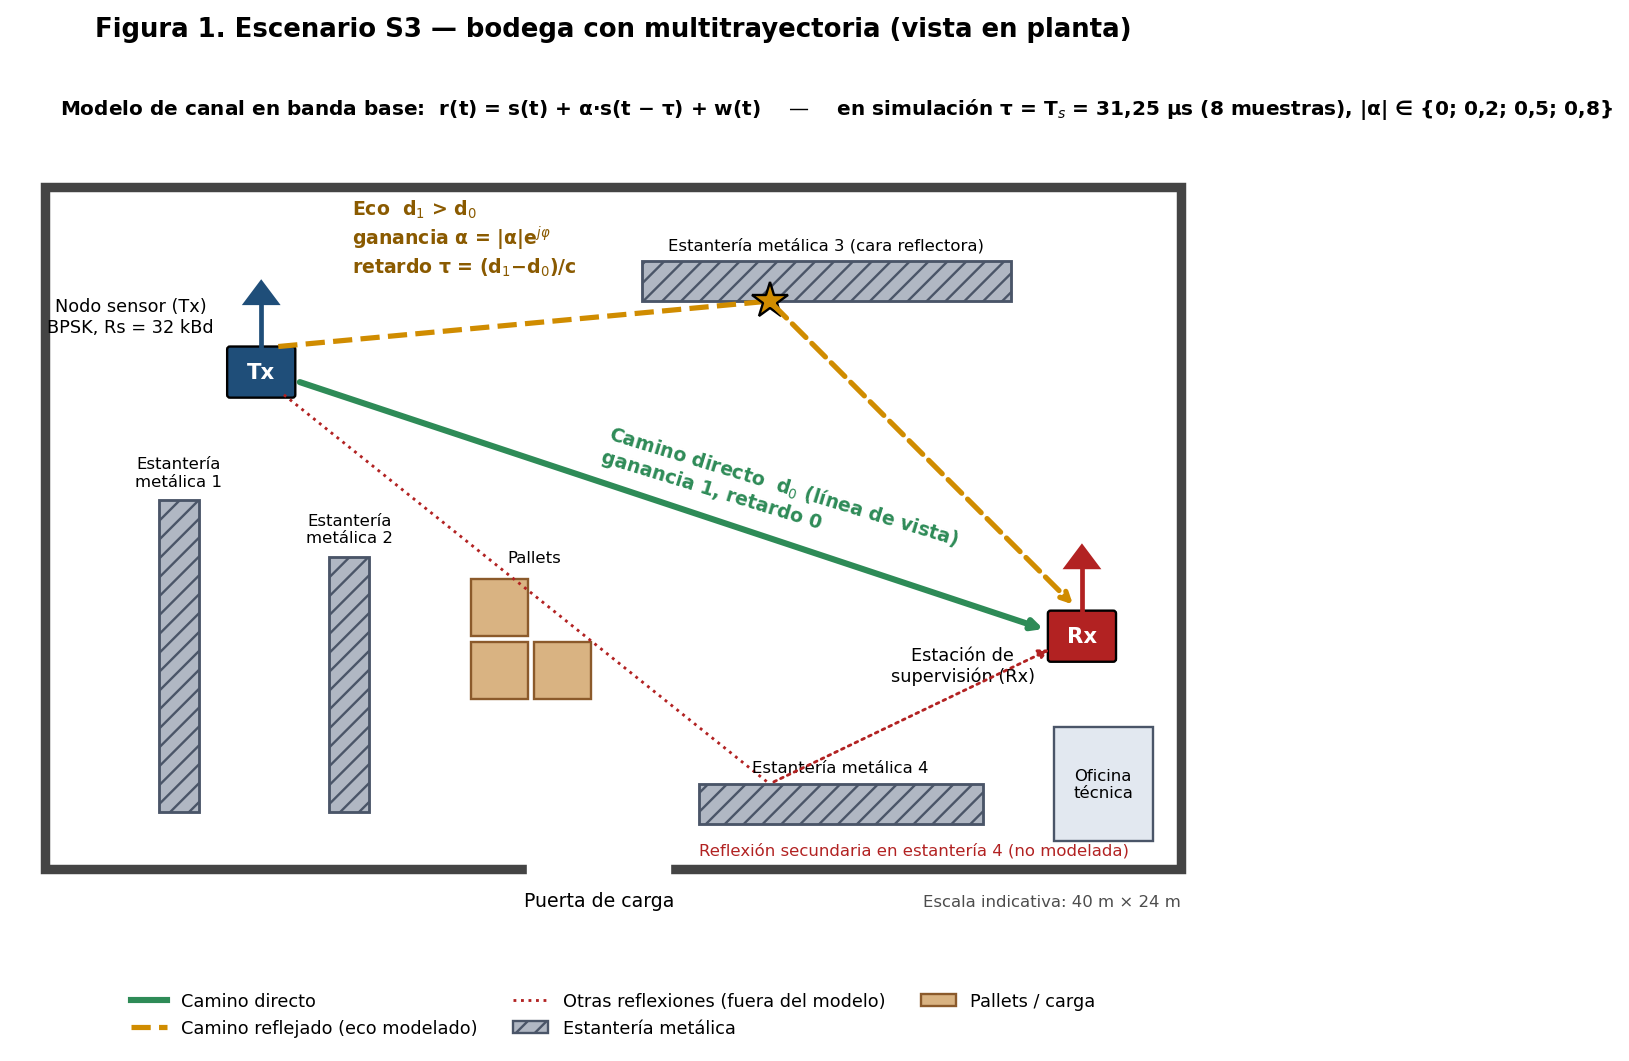
\includegraphics[width=0.78\textwidth]{Fig1_Escenario_S3_bodega.png}
\caption{Escenario S3 (imagen contextual propia): bodega con estanterías metálicas, Tx y Rx con antenas, camino directo, eco modelado y reflexión secundaria no modelada.}
\label{fig:escenario}
\end{figure*}

\subsection{Decisión de modulación y parámetros}
Se eligió BPSK ($M=2$) porque la información de telemetría es de baja tasa y conviene la máxima separación entre símbolos ($d=2$ con energía unitaria). Así, el único mecanismo de degradación observable es el eco. Se consideró QPSK, que duplica $R_b$ con la misma $R_s$, pero la cuadratura y la fase del eco mezclarían los ejes I/Q y harían más difícil atribuir la degradación al eco. Las relaciones del sistema \cite{guia1,guia2} son
\begin{align}
    k&=\log_2 M = 1~\text{bit/símbolo}, \qquad R_b=R_s\,k=32~\text{kb/s},\label{eq:rb}\\
    f_s&=R_s\cdot Sps=32\,000\times 8=256~\text{kS/s}.\label{eq:fs}
\end{align}
Con pulso rectangular de duración $T_s$, la DEP de la envolvente compleja es $S(f)\propto\mathrm{sinc}^2(fT_s)$. Su lóbulo principal ocupa $|f|<R_s$, es decir, $BW_{\text{nulo-nulo}}=2R_s=64$~kHz, con nulos en múltiplos de 32~kHz. La relación $BW\approx(1+\beta)R_s$ aplica solo a conformación RRC; se mantuvo el pulso rectangular del GRC base, como se decidió en la ficha, para no introducir ISI propia del filtro. Los 32~kb/s superan con amplitud la necesidad de variables de proceso lentas, y $Sps=8$ da resolución suficiente para el ojo y para ubicar el retardo en muestras enteras. La Tabla~\ref{tab:parametros} resume la configuración.

\begin{table}[!t]
\centering
\caption{Parámetros del sistema implementado}
\label{tab:parametros}
\footnotesize
\begin{tabular}{llc}
\toprule
\textbf{Parámetro} & \textbf{Variable GRC} & \textbf{Valor} \\
\midrule
Modulación / tabla & \texttt{tabla\_de\_verdad\_constelacion} & BPSK $(-1, +1)$ \\
Símbolos / bits por símbolo & \texttt{M}, \texttt{bps} & 2 / 1 \\
Tasa de símbolos & \texttt{Rs} & 32~kBd \\
Tasa de bits & \texttt{Rb} & 32~kb/s \\
Muestras por símbolo & \texttt{Sps} & 8 \\
Tasa de muestreo & \texttt{samp\_rate} & 256~kS/s \\
Pulso Tx / filtro Rx & \texttt{h}, \texttt{h\_mf} & $[1]\times8$ / $[1/8]\times8$ \\
Retardo del eco & \texttt{D\_eco} & 8 muestras ($31{,}25~\mu$s) \\
Ganancia del eco & \texttt{eco\_alpha}, \texttt{eco\_fase\_deg} & $\{0;0{,}2;0{,}5;0{,}8\}$, $0^\circ$ \\
AWGN de referencia & \texttt{noise\_amp} & 0,10 \\
\bottomrule
\end{tabular}
\end{table}

\subsection{Arquitectura implementada en GNU Radio}
Se partió de una copia de \texttt{Modulaciones\_basadas\_en\_constelaciones\_AWGN.grc} (Figura~\ref{fig:grc_base}), que se conservó intacta, y se creó \texttt{S3\_Multitrayectoria\_BPSK\_Grupo5.grc} (Figuras~\ref{fig:bloques} y \ref{fig:grc_mod}). Las modificaciones fueron:
\begin{itemize}
    \item \textbf{Transmisor:} tabla BPSK $(-1+0j, 1+0j)$; se conservan la fuente aleatoria, el empaquetado, el mapeo y el conformador rectangular por interpolación.
    \item \textbf{Canal S3:} \emph{Delay} de \texttt{D\_eco}$=Sps$ muestras y \emph{Multiply Const} por \texttt{alpha\_c}$=|\alpha|e^{j\varphi}$, sumados al camino directo; después se suma la fuente AWGN original. Un \emph{QT GUI Chooser} selecciona las pruebas A--D.
    \item \textbf{Receptor (Guía~2):} (1) filtro acoplado FIR $h_{mf}=[1/8]\times8$, coherente con el pulso rectangular (integrar y descargar); (2) \emph{QT GUI Eye Sink} sobre la parte real para ubicar el instante de máxima apertura; (3) \emph{Keep One in N} con $N=8$, que conserva la muestra $8k+7$, justo al final del símbolo, donde el filtro acoplado alcanza su pico (verificado numéricamente); (4) decisión con \emph{Complex to Real} y \emph{Binary Slicer} con umbral 0; (5) validación: XOR entre bits Tx retardados \texttt{delay\_bits} y bits Rx, promedio móvil de $N_{ber}=20\,000$ bits y comparación gráfica de bits.
\end{itemize}
A la salida del filtro acoplado, la muestra de decisión es
\begin{equation}
    y_k = s_k + \alpha\, s_{k-1} + n_k, \qquad \sigma_n^2=\frac{N_0R_s}{2},
    \label{eq:yk}
\end{equation}
de modo que cada punto BPSK se desdobla en $\pm1\pm\alpha$ y la distancia mínima al umbral pasa de 1 a $1-|\alpha|$.

\begin{figure}[!t]
\centering
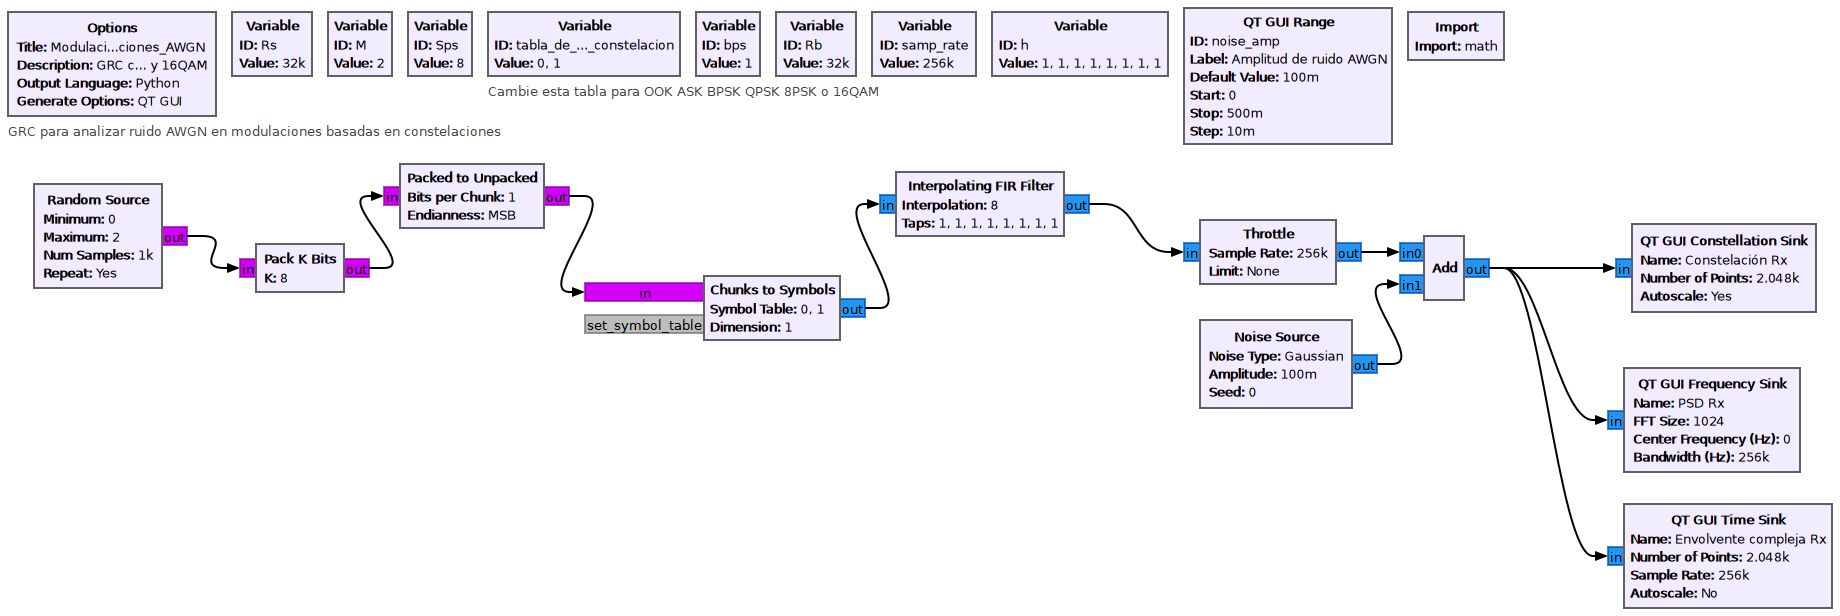
\includegraphics[width=\columnwidth]{GRC_base_original_constelaciones_AWGN.png}
\caption{GRC base del curso (\texttt{Modulaciones\_basadas\_en\_constelaciones\_AWGN.grc}), sin modificar; captura de GNU Radio Companion 3.10.12.}
\label{fig:grc_base}
\end{figure}

\begin{figure*}[!t]
\centering
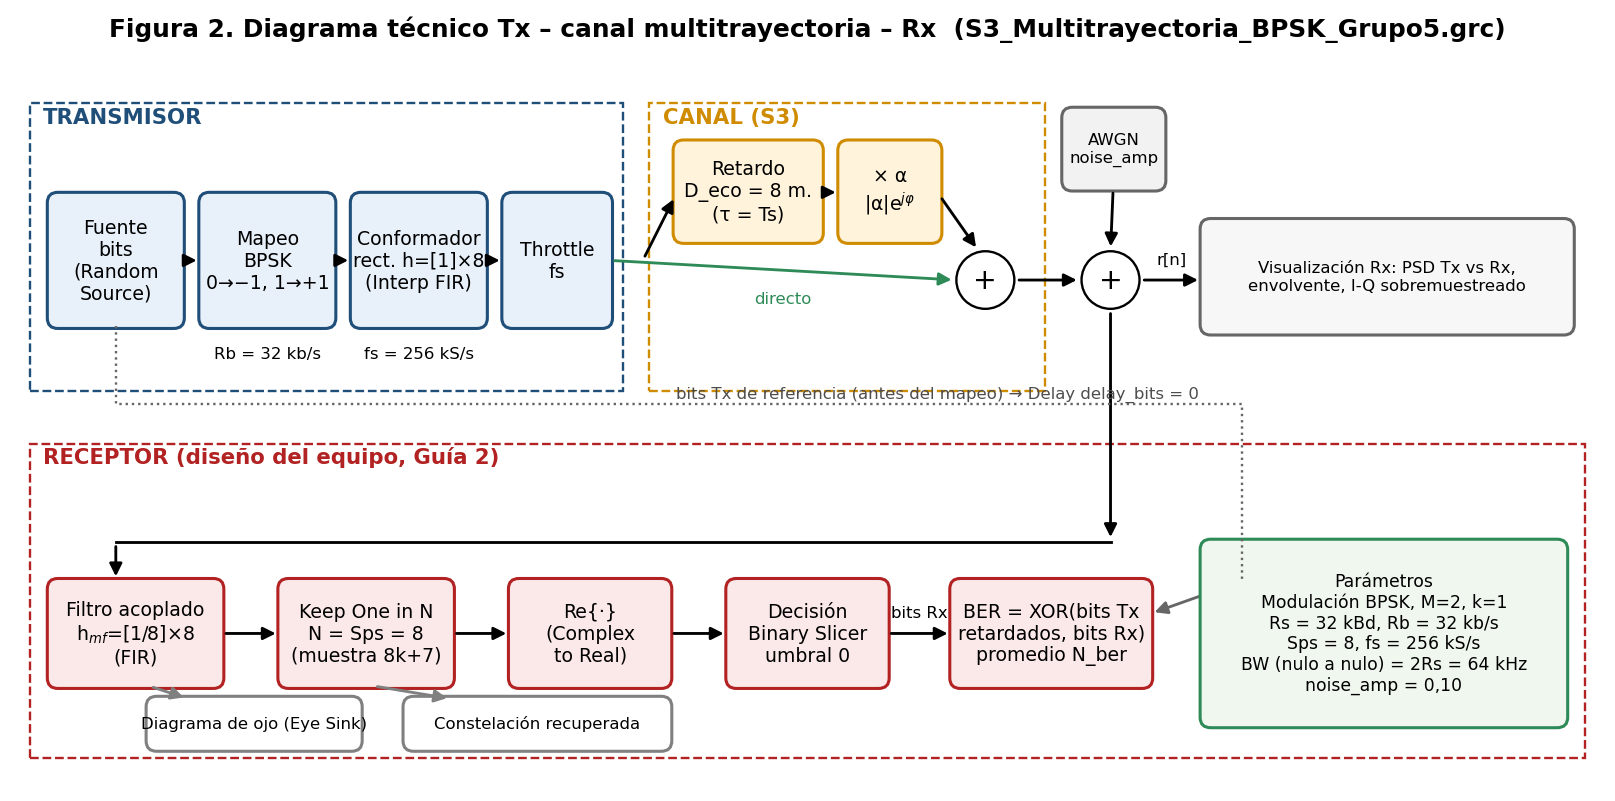
\includegraphics[width=0.92\textwidth]{Fig2_Diagrama_Tx_Canal_Rx.png}
\caption{Diagrama técnico del sistema Tx -- canal multitrayectoria -- Rx con sus parámetros.}
\label{fig:bloques}
\end{figure*}

\begin{figure*}[!t]
\centering
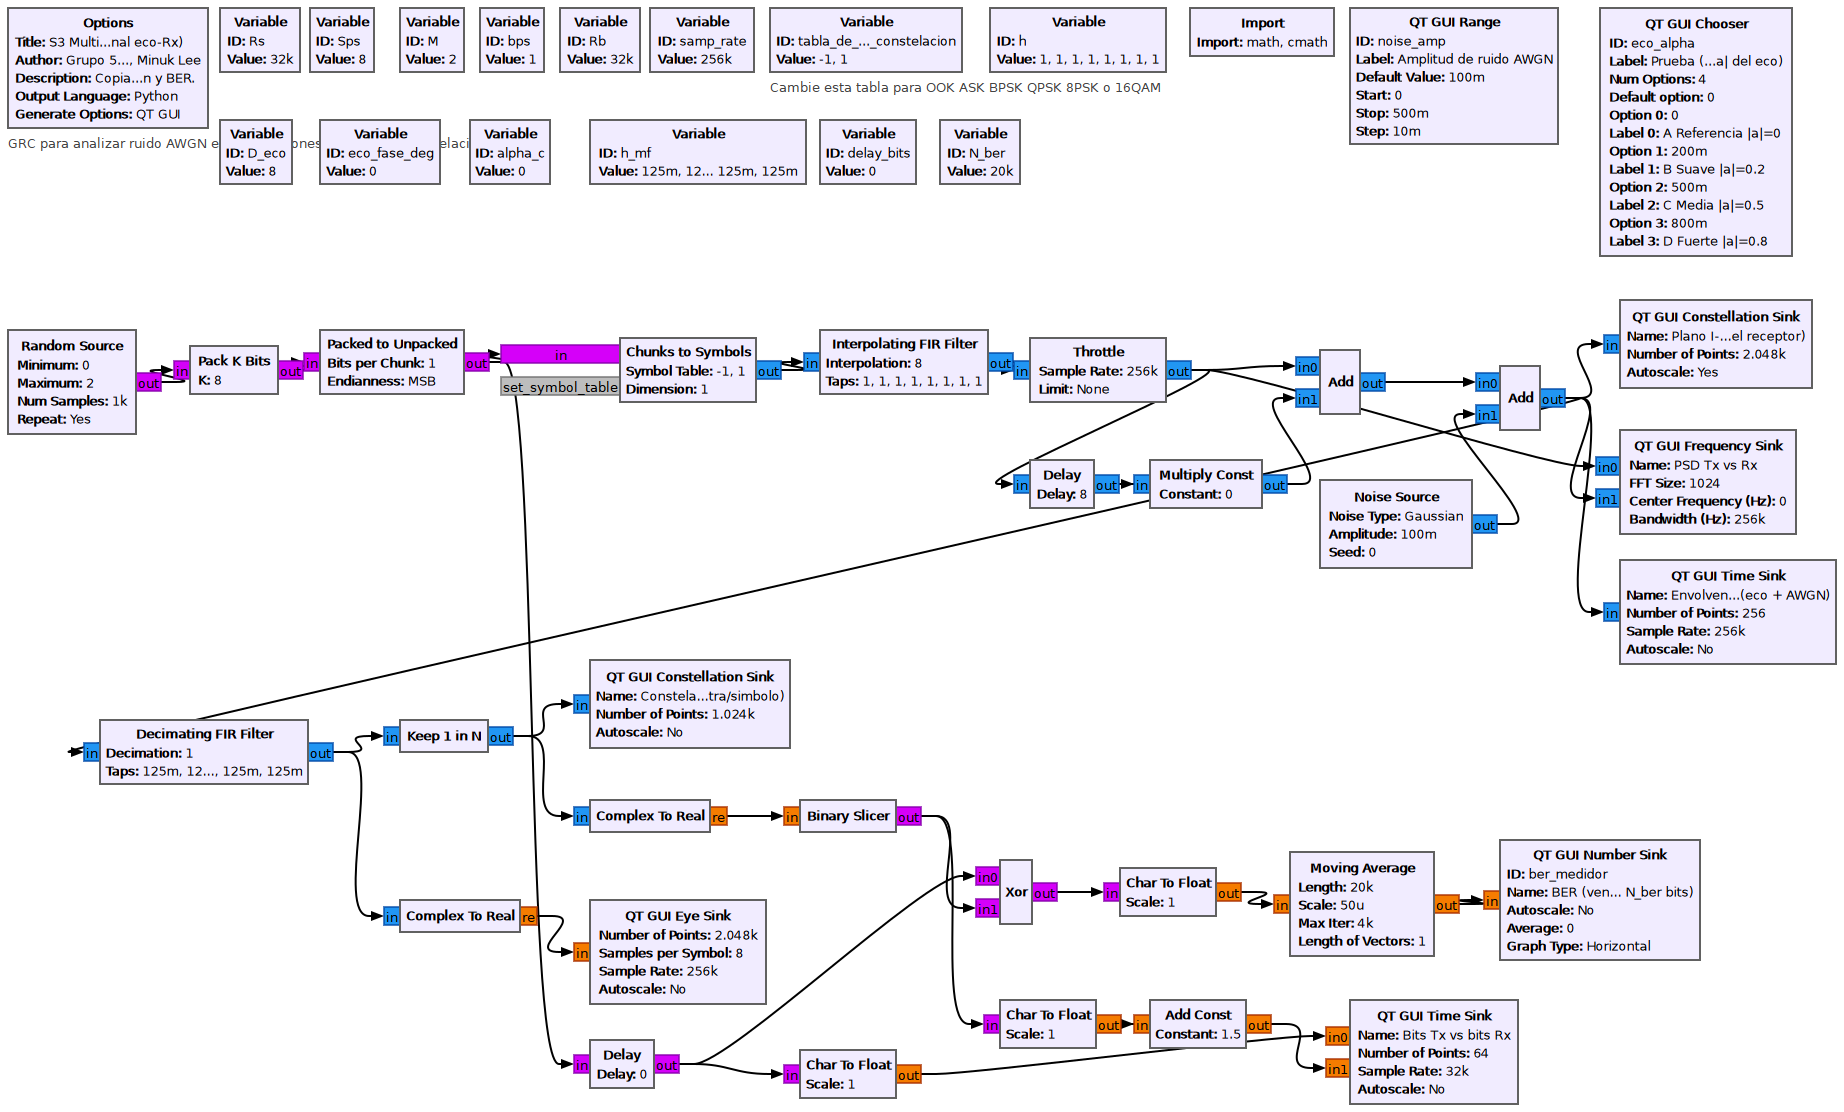
\includegraphics[width=0.92\textwidth]{GRC_S3_Multitrayectoria_BPSK_Grupo5.png}
\caption{GRC modificado \texttt{S3\_Multitrayectoria\_BPSK\_Grupo5.grc} (captura de pantalla de GRC~3.10.12 en el equipo del grupo): Tx BPSK, canal eco (Delay + Multiply Const + Add), AWGN y receptor.}
\label{fig:grc_mod}
\end{figure*}

\subsection{Procedimiento experimental}
Se realizaron cuatro pruebas cambiando solo $|\alpha|$ (Tabla~\ref{tab:pruebas}); $\tau$, la fase, el ruido, $R_s$, $Sps$ y $f_s$ se mantuvieron constantes. Para exportar datos se generó una variante sin GUI del mismo flujograma, en la que los sinks QT se sustituyen por \emph{File Sinks} y el Throttle por un \emph{Head} de 200\,000 bits. Esa variante se ejecutó con GNU Radio 3.10.9 en Linux, y las gráficas se obtuvieron de los datos crudos. El GRC con GUI se ejecutó además en GNU Radio 3.10.12 (radioconda, Windows) en el equipo del grupo, con resultados visuales idénticos (Anexo~\ref{app:evidencias}).

\subsection{Instrumentación BER (Fase 4)}
Se integraron \texttt{e\_EbN0\_Sweep} y \texttt{e\_BER\_Curve} \cite{guia4} en \texttt{S3\_BER\_Multitrayectoria\_BPSK\_Grupo5.grc}. El barrido reemplaza a la fuente AWGN fija y se ubica justo antes del filtro acoplado, con $bb\_rate=f_s=256$~kS/s y $R_b=32\,000$~b/s. La referencia Tx se toma de los bits antes del mapeo, y los bits Rx a la salida del \emph{Binary Slicer}. El ruido agregado cumple
\begin{equation}
    P_n=\frac{P_s\,f_s}{R_b\,(E_b/N_0)},
    \label{eq:pn}
\end{equation}
donde $P_s$ es la potencia medida a la entrada del barrido, que incluye el eco: $P_s=1+|\alpha|^2+2|\alpha|\rho_1$, con $\rho_1$ la correlación entre símbolos adyacentes. La BER teórica de referencia, obtenida de \eqref{eq:yk} y \eqref{eq:pn} con $\rho_1\approx0$, es
\begin{equation}
    P_b=\tfrac12 Q\!\left(\!\sqrt{\tfrac{2\gamma}{P_s}}(1+|\alpha|)\!\right)+\tfrac12 Q\!\left(\!\sqrt{\tfrac{2\gamma}{P_s}}(1-|\alpha|)\!\right),
    \label{eq:pb}
\end{equation}
con $\gamma=E_b/N_0$; para $\alpha=0$ se reduce a $Q(\sqrt{2\gamma})$ \cite{proakis2008}. Se usaron $E_bN_0\in[0,14]$~dB en pasos de 1~dB, \texttt{bits\_por\_punto}$=100\,000$, \texttt{bits\_guardia}$=1000$ y dos barridos completos por cada $|\alpha|$.

Al integrar la plantilla se encontraron y corrigieron dos errores que impedían usarla en GNU Radio 3.10, comprobados en GRC~3.10.12 del equipo (Anexo~\ref{app:correcciones}): (i) \texttt{e\_BER\_Curve} heredaba de \texttt{gr.sync\_decimator}, que en 3.10 es la clase C++ enlazada y no una clase de bloque Python, por lo que GRC no reconoce el bloque; se cambió a \texttt{gr.decim\_block}; (ii) \texttt{e\_BER\_CSV} usa \texttt{\_\_file\_\_}, que no existe cuando GRC instancia el bloque para validarlo; se añadió un respaldo a \texttt{Path.cwd()}. Además, se ligaron los parámetros de \texttt{e\_BER\_Curve} a las variables (\texttt{delay\_bits}, etc.), que en la plantilla no estaban conectados.

\textbf{Alineación Tx/Rx.} En condición limpia (prueba A, $E_b/N_0\approx29$~dB) se evaluó la BER para \texttt{delay\_bits}$=0\ldots8$. Solo con \texttt{delay\_bits}$=0$ se obtuvo BER $=0$ (0 errores en 200\,000 bits); para los demás valores la BER es $\approx0{,}5$. Esto es coherente con la temporización: el filtro acoplado y la decimación no introducen retardo entero de símbolo.

\subsection{Preparación para hardware (Fase 3)}
Se generaron \texttt{S3\_BPSK\_Grupo5\_HackRF\_TX/RX.grc} con los bloques \emph{Osmocom Sink/Source} del archivo de referencia del curso (fc$=960$~MHz, LO desplazado 200~kHz, \texttt{radio\_rate}$=2$~MS/s). La adaptación de tasa es $radio\_rate=bb\_rate\cdot125/16$ y la inversa en Rx, sin cambiar $R_s$. Se retiró el Throttle. Como el hardware no garantiza sincronismo, el Rx incorpora AGC, \emph{Symbol Sync} (Gardner) \cite{gnuradio_symsync} y lazo de Costas de orden~2. Esta cadena se verificó en simulación con desfases de 0 a 3~kHz, error de reloj de 0 a 100~ppm y ruido, y en todos los casos se obtuvieron 0 errores en 100\,000 bits, con la ambigüedad de fase de $180^\circ$ propia de BPSK (bits invertidos), que debe resolverse con una secuencia conocida o con codificación diferencial. La configuración no se probó con hardware porque el radio no estaba disponible.

\section{Resultados y análisis}

\subsection{Tabla de pruebas}
La Tabla~\ref{tab:pruebas} resume las cuatro condiciones con los valores exactos y las métricas medidas a partir de los datos exportados por GNU Radio (200\,000 bits por prueba). La potencia de ruido medida ($\sigma^2=0{,}010$) confirma \texttt{noise\_amp}$=0{,}10$, equivalente a $E_b/N_0\approx29$~dB respecto al camino directo. La potencia recibida coincide con $1+|\alpha|^2+2|\alpha|\rho_1+\sigma^2$ con error menor de $10^{-3}$. El término $\rho_1$ es la autocorrelación de la secuencia de prueba (la fuente del curso repite 1000 bits) y vale entre $-0{,}056$ y $0{,}064$ según la ejecución.

\begin{table}[!t]
\centering
\caption{Pruebas A--D ($\tau=T_s$, fase $0^\circ$, \texttt{noise\_amp}$=0{,}10$, 200\,000 bits)}
\label{tab:pruebas}
\footnotesize
\setlength{\tabcolsep}{3pt}
\begin{tabular}{lccccc}
\toprule
\textbf{Prueba} & $|\alpha|$ & \textbf{Ojo medido} & \textbf{Ojo teórico} & \textbf{EVM} & \textbf{Errores} \\
 & & [V] & $2(1-|\alpha|)$ & [\%] & \\
\midrule
A Referencia & 0   & 1,84 & 2,0 & 3,5  & 0 \\
B Suave      & 0,2 & 1,46 & 1,6 & 20,3 & 0 \\
C Media      & 0,5 & 0,86 & 1,0 & 50,1 & 0 \\
D Fuerte     & 0,8 & 0,26 & 0,4 & 80,1 & 0 \\
\bottomrule
\end{tabular}
\\[2pt]\raggedright\scriptsize Ojo medido: diferencia entre el percentil 0,1~\% de los ``1'' y el 99,9~\% de los ``0'' en el instante de decisión. EVM respecto a $\pm1$.
\end{table}

\subsection{Densidad espectral de potencia}
En la referencia (Figura~\ref{fig:psd}a), la PSD Tx y la Rx coinciden en la forma $\mathrm{sinc}^2$: lóbulo principal de $\pm32$~kHz ($BW_{\text{nulo-nulo}}=64$~kHz) y nulos en múltiplos de $R_s$. El ruido solo eleva el piso cerca de los nulos. Con eco fuerte (Figura~\ref{fig:psd}b), la PSD recibida queda modulada por $|H(f)|^2$: aumenta en DC y en $\pm32$~kHz y cae en $\pm16$~kHz ($f=1/2\tau$), donde la réplica llega en contrafase. La Figura~\ref{fig:hf} compara el cociente $P_{rx}/P_{tx}$ medido con $|1+\alpha e^{-j2\pi fT_s}|^2$. La coincidencia es casi total: mínimos de $-1{,}9$, $-6{,}0$ y $-14{,}0$~dB para $|\alpha|=0{,}2$; 0,5 y 0,8. Los picos en $\pm32$~kHz son artefactos del cociente, porque allí la PSD Tx tiene nulos. La PSD muestra así que el eco no agrega potencia en otra banda: \emph{redistribuye} la energía dentro de la banda útil. Ese es el desvanecimiento selectivo en frecuencia que, en el dominio del tiempo, se manifiesta como ISI.

\begin{figure}[!t]
\centering
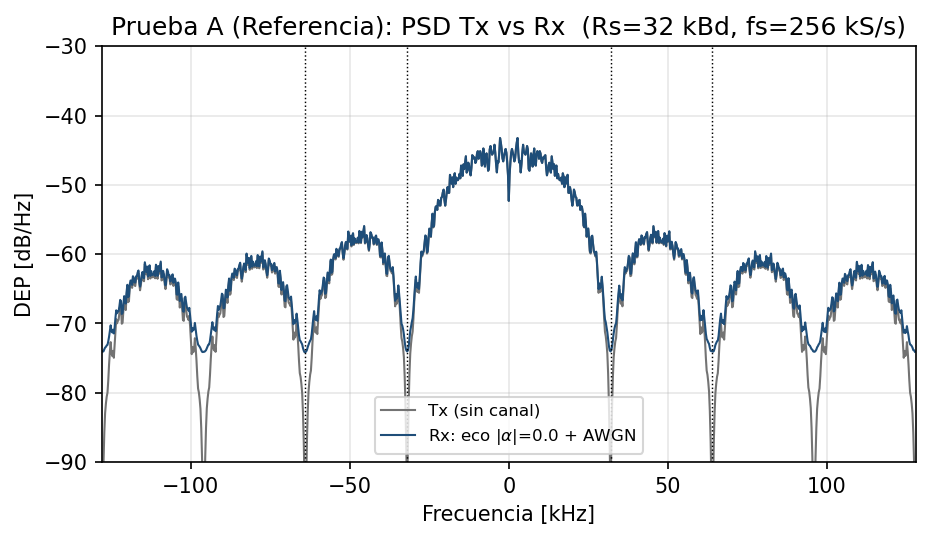
\includegraphics[width=\columnwidth]{PSD_prueba_A.png}\\[-1pt]
{\scriptsize (a)}\\
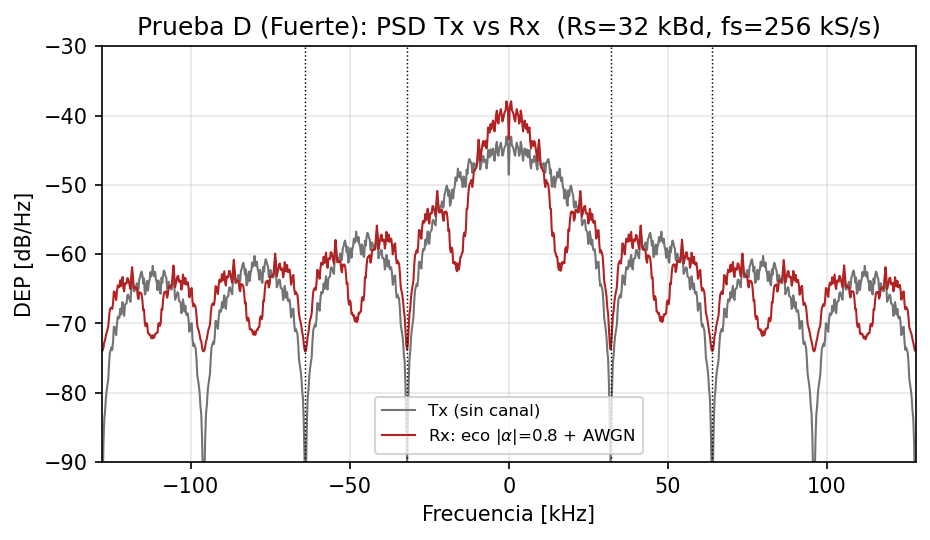
\includegraphics[width=\columnwidth]{PSD_prueba_D.png}\\[-1pt]
{\scriptsize (b)}
\caption{PSD Tx vs.\ Rx (Welch, 1024 puntos): (a) prueba A, referencia; (b) prueba D, $|\alpha|=0{,}8$.}
\label{fig:psd}
\end{figure}

\begin{figure}[!t]
\centering
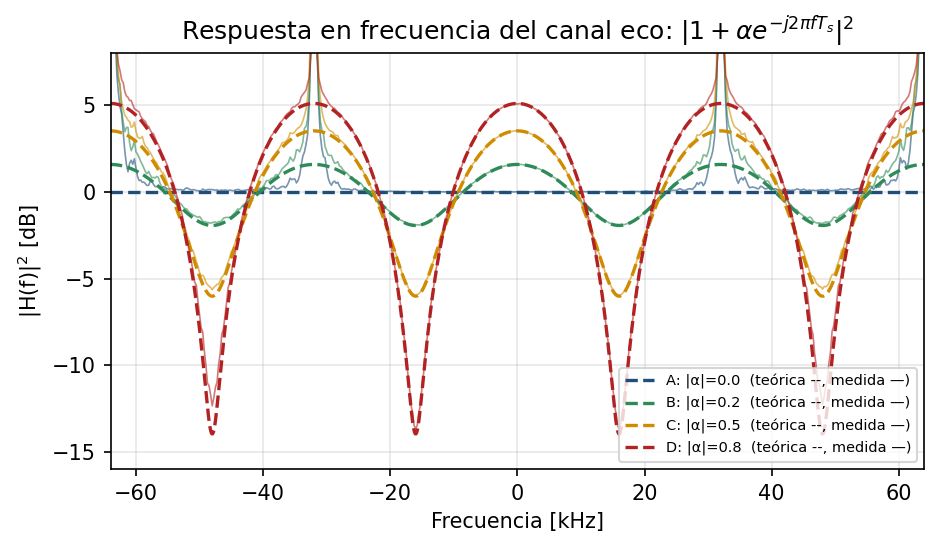
\includegraphics[width=\columnwidth]{Respuesta_frecuencia_canal.png}
\caption{Respuesta en frecuencia del canal: cociente medido $P_{rx}/P_{tx}$ (línea continua) frente al modelo $|1+\alpha e^{-j2\pi fT_s}|^2$ (línea discontinua).}
\label{fig:hf}
\end{figure}

\subsection{Señal temporal}
En la prueba C (Figura~\ref{fig:temporal}), cada símbolo de la señal recibida toma el valor $s_k+0{,}5\,s_{k-1}$. Cuando dos bits consecutivos son iguales el nivel sube a $\pm1{,}5$, y cuando cambian baja a $\pm0{,}5$. La salida del filtro acoplado integra cada símbolo y alcanza su valor final en la muestra $8k+7$ (puntos negros). Ese es el instante que selecciona \emph{Keep One in N}. El efecto del eco, por tanto, es visible en el tiempo: los niveles dependen del símbolo anterior, que es la definición de ISI.

\begin{figure}[!t]
\centering
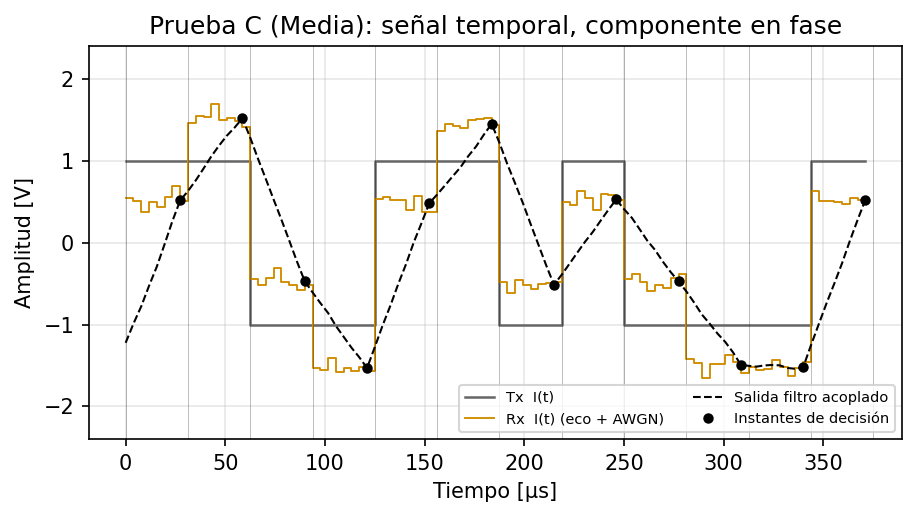
\includegraphics[width=\columnwidth]{Temporal_prueba_C.png}
\caption{Prueba C ($|\alpha|=0{,}5$): componente en fase Tx, Rx y salida del filtro acoplado con los instantes de decisión.}
\label{fig:temporal}
\end{figure}

\subsection{Constelación y diagrama de ojo}
Las Figuras~\ref{fig:const} y \ref{fig:ojo} muestran la evolución de las cuatro pruebas.
\textbf{A (referencia):} dos nubes compactas en $\pm1$ (EVM 3,5~\%) y un ojo abierto con apertura 1,84~V, limitada solo por el ruido. Es la línea base del receptor.
\textbf{B (suave):} cada nube se divide en dos, en $\pm1\pm0{,}2$, y el ojo baja a 1,46~V. La degradación comienza, pero el margen sigue siendo amplio, y el AWGN de referencia no produce errores.
\textbf{C (media):} los cuatro niveles $\pm0{,}5$ y $\pm1{,}5$ quedan bien separados. El ojo se reduce a la mitad (0,86~V), así que cualquier aumento del ruido se traduce rápidamente en errores. Esta es la condición principal de análisis porque muestra con claridad el mecanismo de ISI.
\textbf{D (fuerte):} los niveles internos $\pm0{,}2$ quedan a solo 0,2~V del umbral y el ojo casi se cierra (0,26~V). Con \texttt{noise\_amp}$=0{,}10$ todavía no hay errores, porque la desviación del ruido tras el filtro es $\approx0{,}025$~V, pero el sistema queda en estrés: la BER depende ahora casi por completo del margen residual $1-|\alpha|$.

Como resume la Figura~\ref{fig:apertura}, la apertura medida sigue la recta teórica $2(1-|\alpha|)$, desplazada unos 0,15~V por el ruido. Esto confirma la hipótesis: el eco no rota ni dispersa la constelación al azar, sino que la \emph{desdobla} de forma determinista según el símbolo anterior.

\begin{figure*}[!t]
\centering
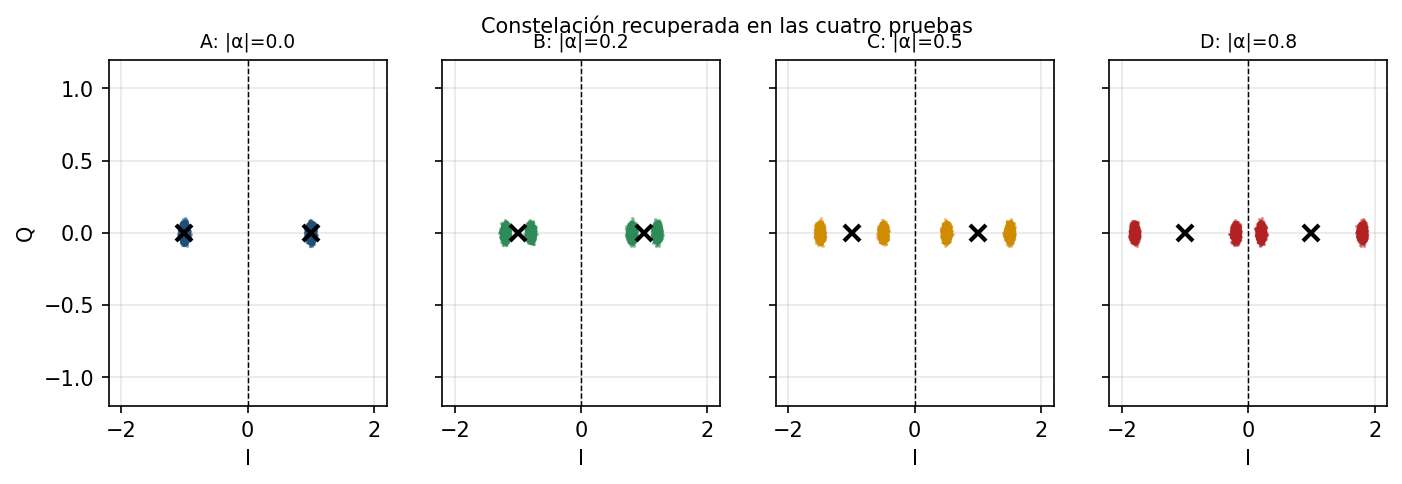
\includegraphics[width=0.9\textwidth]{Constelaciones_comparacion_ABCD.png}
\caption{Constelación recuperada (1 muestra/símbolo) en las pruebas A--D. Las cruces son los símbolos ideales $\pm1$.}
\label{fig:const}
\end{figure*}

\begin{figure*}[!t]
\centering
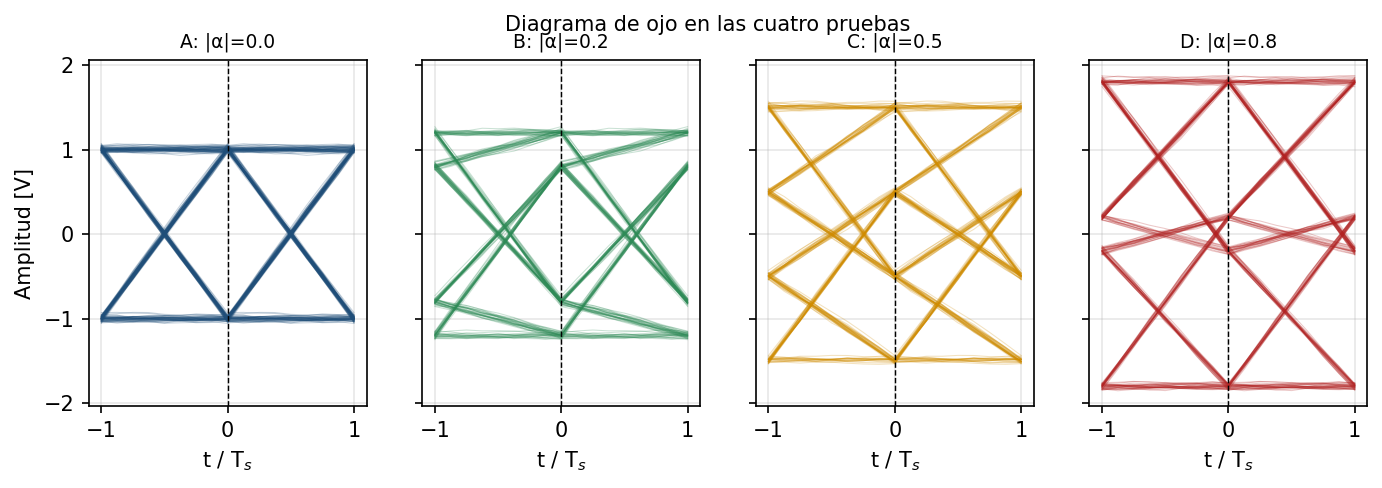
\includegraphics[width=0.9\textwidth]{Ojos_comparacion_ABCD.png}
\caption{Diagrama de ojo a la salida del filtro acoplado (parte real) en las pruebas A--D; $t=0$ es el instante de decisión.}
\label{fig:ojo}
\end{figure*}

\begin{figure}[!t]
\centering
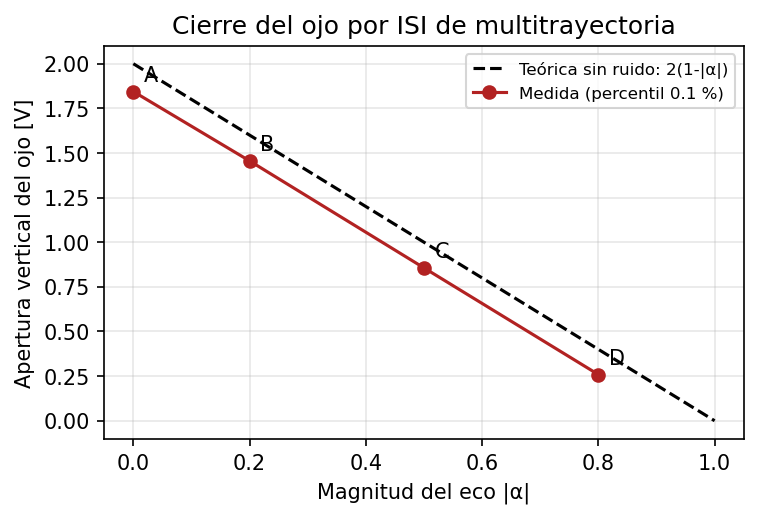
\includegraphics[width=0.85\columnwidth]{Apertura_ojo_vs_alpha.png}
\caption{Apertura vertical del ojo medida frente a la teórica sin ruido $2(1-|\alpha|)$.}
\label{fig:apertura}
\end{figure}

\subsection{Curva BER vs.\ $E_b/N_0$}
La Figura~\ref{fig:ber} presenta las curvas obtenidas directamente de los archivos \texttt{curva\_BER.csv} generados por el instrumento, sin editar. Para $\alpha=0$, la BER medida sigue $Q(\sqrt{2E_b/N_0})$: $7{,}9\times10^{-2}$ a 0~dB (teoría $7{,}9\times10^{-2}$), $8{,}1\times10^{-4}$ a 7~dB (teoría $7{,}7\times10^{-4}$) y $3{,}5\times10^{-5}$ a 9~dB. A partir de 10~dB no se detectaron errores en 200\,000 bits por punto. Esto no significa BER $=0$: indica $BER<1{,}5\times10^{-5}$, que el instrumento grafica como la cota $3/N$. Una ejecución independiente en el equipo del grupo (GRC 3.10.12, Windows) reprodujo la curva con diferencias dentro de la dispersión estadística (p.~ej., $7{,}2\times10^{-4}$ a 7~dB).

Con eco, las curvas se desplazan a la derecha y se aplanan, en concordancia con \eqref{eq:pb} (Tabla~\ref{tab:penalizacion}). El término $(1-|\alpha|)$ domina la BER, y además el eco ``gasta'' energía: $E_b$ se mide sobre la potencia total $1+|\alpha|^2$, pero solo la parte coherente ayuda a la decisión. Según el criterio del proyecto (penalización $\le2$~dB a BER $=10^{-3}$), el eco suave es tolerable sin ecualización (1,4~dB), el eco medio no lo es (6,3~dB) y con el eco fuerte la curva no alcanza $10^{-3}$ en todo el barrido. La teoría predice 22,3~dB, es decir, una penalización de unos 15,5~dB. Las diferencias entre medición y teoría están dentro de $\pm0{,}05$~dB, lo que valida tanto la integración del instrumento como la alineación \texttt{delay\_bits}$=0$.

\begin{figure}[!t]
\centering
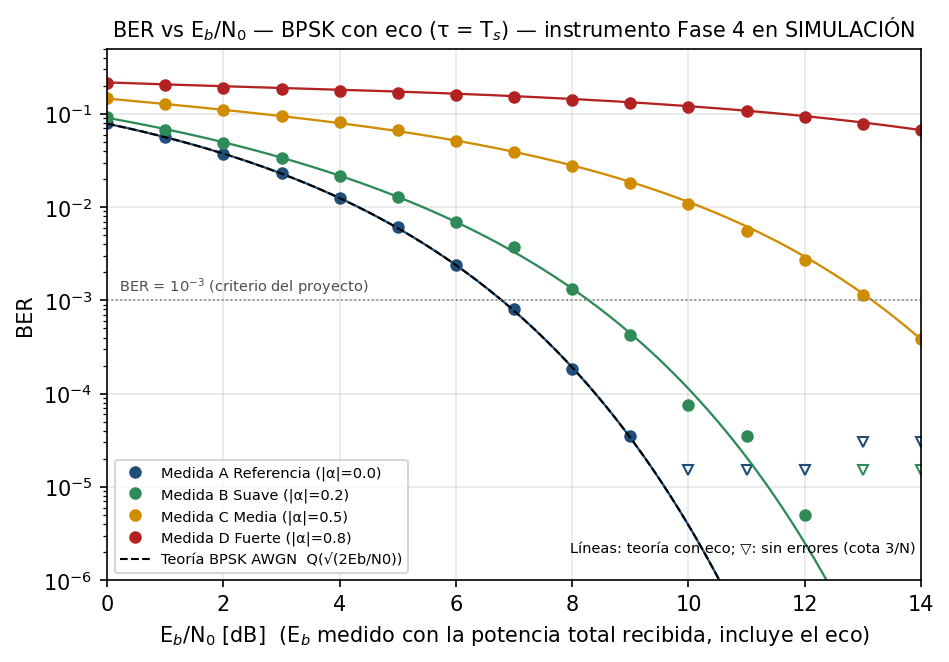
\includegraphics[width=\columnwidth]{BER_vs_EbN0_eco.png}
\caption{BER vs.\ $E_b/N_0$ medida con el instrumento de la Fase~4 (simulación) para las cuatro pruebas, con la teoría de \eqref{eq:pb} y la curva BPSK en AWGN.}
\label{fig:ber}
\end{figure}

\begin{table}[!t]
\centering
\caption{$E_b/N_0$ requerido para BER $=10^{-3}$ y penalización por eco}
\label{tab:penalizacion}
\footnotesize
\begin{tabular}{lcccc}
\toprule
$|\alpha|$ & \textbf{Medido} [dB] & \textbf{Teórico} [dB] & \textbf{Penalización} [dB] & \textbf{$\le$2 dB} \\
\midrule
0   & 6,80 & 6,79 & 0 (ref.) & Sí \\
0,2 & 8,24 & 8,28 & 1,44 & Sí \\
0,5 & 13,11 & 13,16 & 6,31 & No \\
0,8 & $>14$ & 22,3 & $\approx15{,}5$ (teórica) & No \\
\bottomrule
\end{tabular}
\end{table}

\subsection{Observaciones de la verificación}
(i) En GRC~3.10.12 (Windows), el \emph{QT GUI Vector Sink} de la plantilla no redibujó la curva durante la ejecución, aunque el bloque CSV, conectado a la misma salida, guardó correctamente los valores. Por ello se tomó como evidencia el CSV, que es el archivo que exige la guía. (ii) La fuente de bits del curso repite una secuencia de 1000 bits, lo que introduce una pequeña correlación $\rho_1$ entre símbolos y explica las variaciones de potencia recibida entre ejecuciones. (iii) El modelo considera un único eco con fase $0^\circ$, el peor caso en fase. Con otra fase, parte del eco cae en la componente Q, y en BPSK el ojo del eje I se cierra solo en $|\alpha|\cos\varphi$.

\section{Conclusiones}

\begin{enumerate}
    \item Con BPSK y pulso rectangular ($R_s=32$~kBd, $R_b=32$~kb/s, $Sps=8$, $f_s=256$~kS/s, $BW_{\text{nulo-nulo}}=64$~kHz), el único mecanismo de degradación observado fue el eco. Esto permitió atribuirle sin ambigüedad cada cambio en las evidencias.
    \item El eco con $\tau=T_s$ actúa como ISI de un símbolo: desdobla la constelación en $\pm1\pm\alpha$ y reduce la apertura del ojo según $2(1-|\alpha|)$ (1,84; 1,46; 0,86 y 0,26~V medidos para $|\alpha|=0$; 0,2; 0,5 y 0,8). En frecuencia se manifiesta como el peine $|1+\alpha e^{-j2\pi fT_s}|^2$, con mínimos de hasta $-14$~dB en $\pm R_s/2$, lo que confirma la hipótesis planteada.
    \item El receptor de filtro acoplado, con muestreo en la muestra $8k+7$ y decisión por umbral cero, recuperó los bits sin errores en las cuatro pruebas con el ruido de referencia, y en AWGN reprodujo la curva teórica de BPSK con una diferencia de 0,01~dB a BER $=10^{-3}$.
    \item La penalización por eco a BER $=10^{-3}$ fue de 1,4~dB ($|\alpha|=0{,}2$), 6,3~dB ($|\alpha|=0{,}5$) y más de 14~dB ($|\alpha|=0{,}8$; 15,5~dB teórica). Con el criterio de 2~dB, solo el eco suave es aceptable sin ecualización.
    \item Al trasladar este caso a una bodega real, un retardo de unos 100~ns produce ISI solo si $R_s$ es del orden de 10~MBd. Para tasas más altas o ecos fuertes se recomienda un ecualizador adaptativo (LMS/DFE) o modulación multiportadora. Como trabajo futuro quedan la validación con HackRF One, con los archivos ya preparados, y el estudio de la fase del eco y de varios ecos.
\end{enumerate}

% ANEXOS
\appendices

\section{Correcciones a la plantilla BER de la Fase 4}
\label{app:correcciones}
Los archivos originales se conservan sin cambios en \texttt{02\_GNU\_Radio/Archivos\_originales}; las versiones corregidas están en \texttt{Archivos\_modificados}. Al abrir la plantilla original en GRC~3.10.12, \texttt{e\_BER\_Curve} y ``Guardar curva BER en CSV'' se muestran con error (título en rojo) y \texttt{e\_BER\_Curve} no expone parámetros.

\begin{lstlisting}[style=bonito, language=Python, caption={Cambios en \texttt{e\_BER\_Curve} y \texttt{e\_BER\_CSV}}, label={lst:correcciones}]
# e_BER_Curve (original -> corregido)
class blk(gr.sync_decimator):          # no es bloque Python en GR 3.10
class blk(gr.decim_block):             # pasarela Python correcta
    gr.decim_block.__init__(self, name='e_BER_Curve', in_sig=[np.int8, np.int8],
        out_sig=[(np.float32, self.N), (np.float32, self.N)], decim=self.update_every)

# e_BER_CSV (original -> corregido)
self.carpeta = Path(__file__).resolve().parent
try:
    self.carpeta = Path(__file__).resolve().parent
except NameError:   # GRC instancia el bloque sin __file__ al validarlo
    self.carpeta = Path.cwd()
\end{lstlisting}

\section{Evidencias de ejecución en el equipo del grupo}
\label{app:evidencias}
La Figura~\ref{fig:gui_pc} es una captura de pantalla real de la GUI de \texttt{S3\_Multitrayectoria\_BPSK\_Grupo5.grc} ejecutándose en GNU Radio Companion 3.10.12 (radioconda, Windows) con la prueba C seleccionada. La Figura~\ref{fig:grc_ber} muestra el flujograma con la instrumentación BER integrada.

\begin{figure}[!h]
\centering
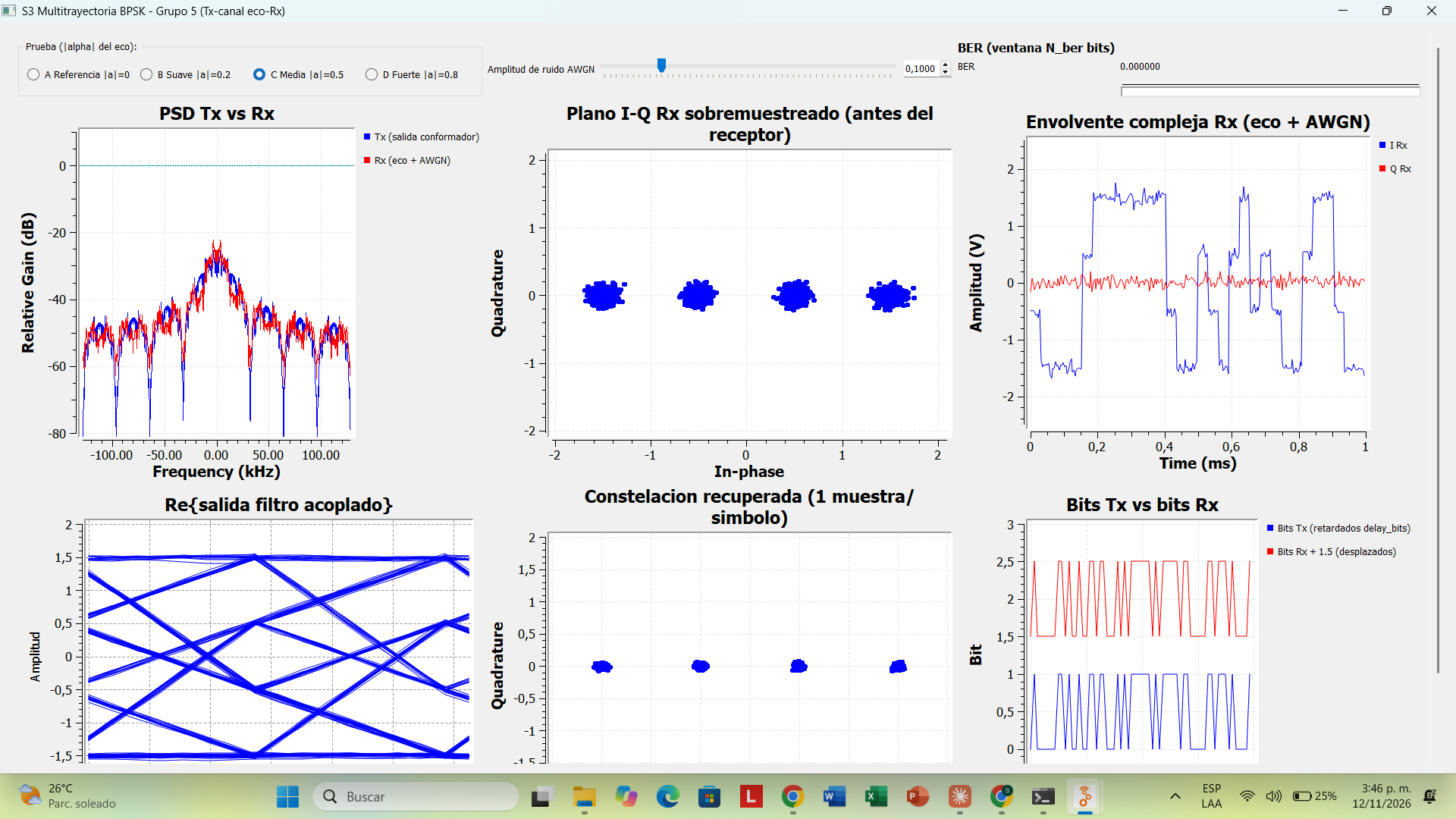
\includegraphics[width=\columnwidth]{PC_GUI_ejecucion_Prueba_C_media.jpg}
\caption{GUI en ejecución (prueba C): PSD Tx/Rx, plano I-Q, envolvente, ojo, constelación recuperada, bits Tx/Rx y medidor de BER.}
\label{fig:gui_pc}
\end{figure}

\begin{figure}[!h]
\centering
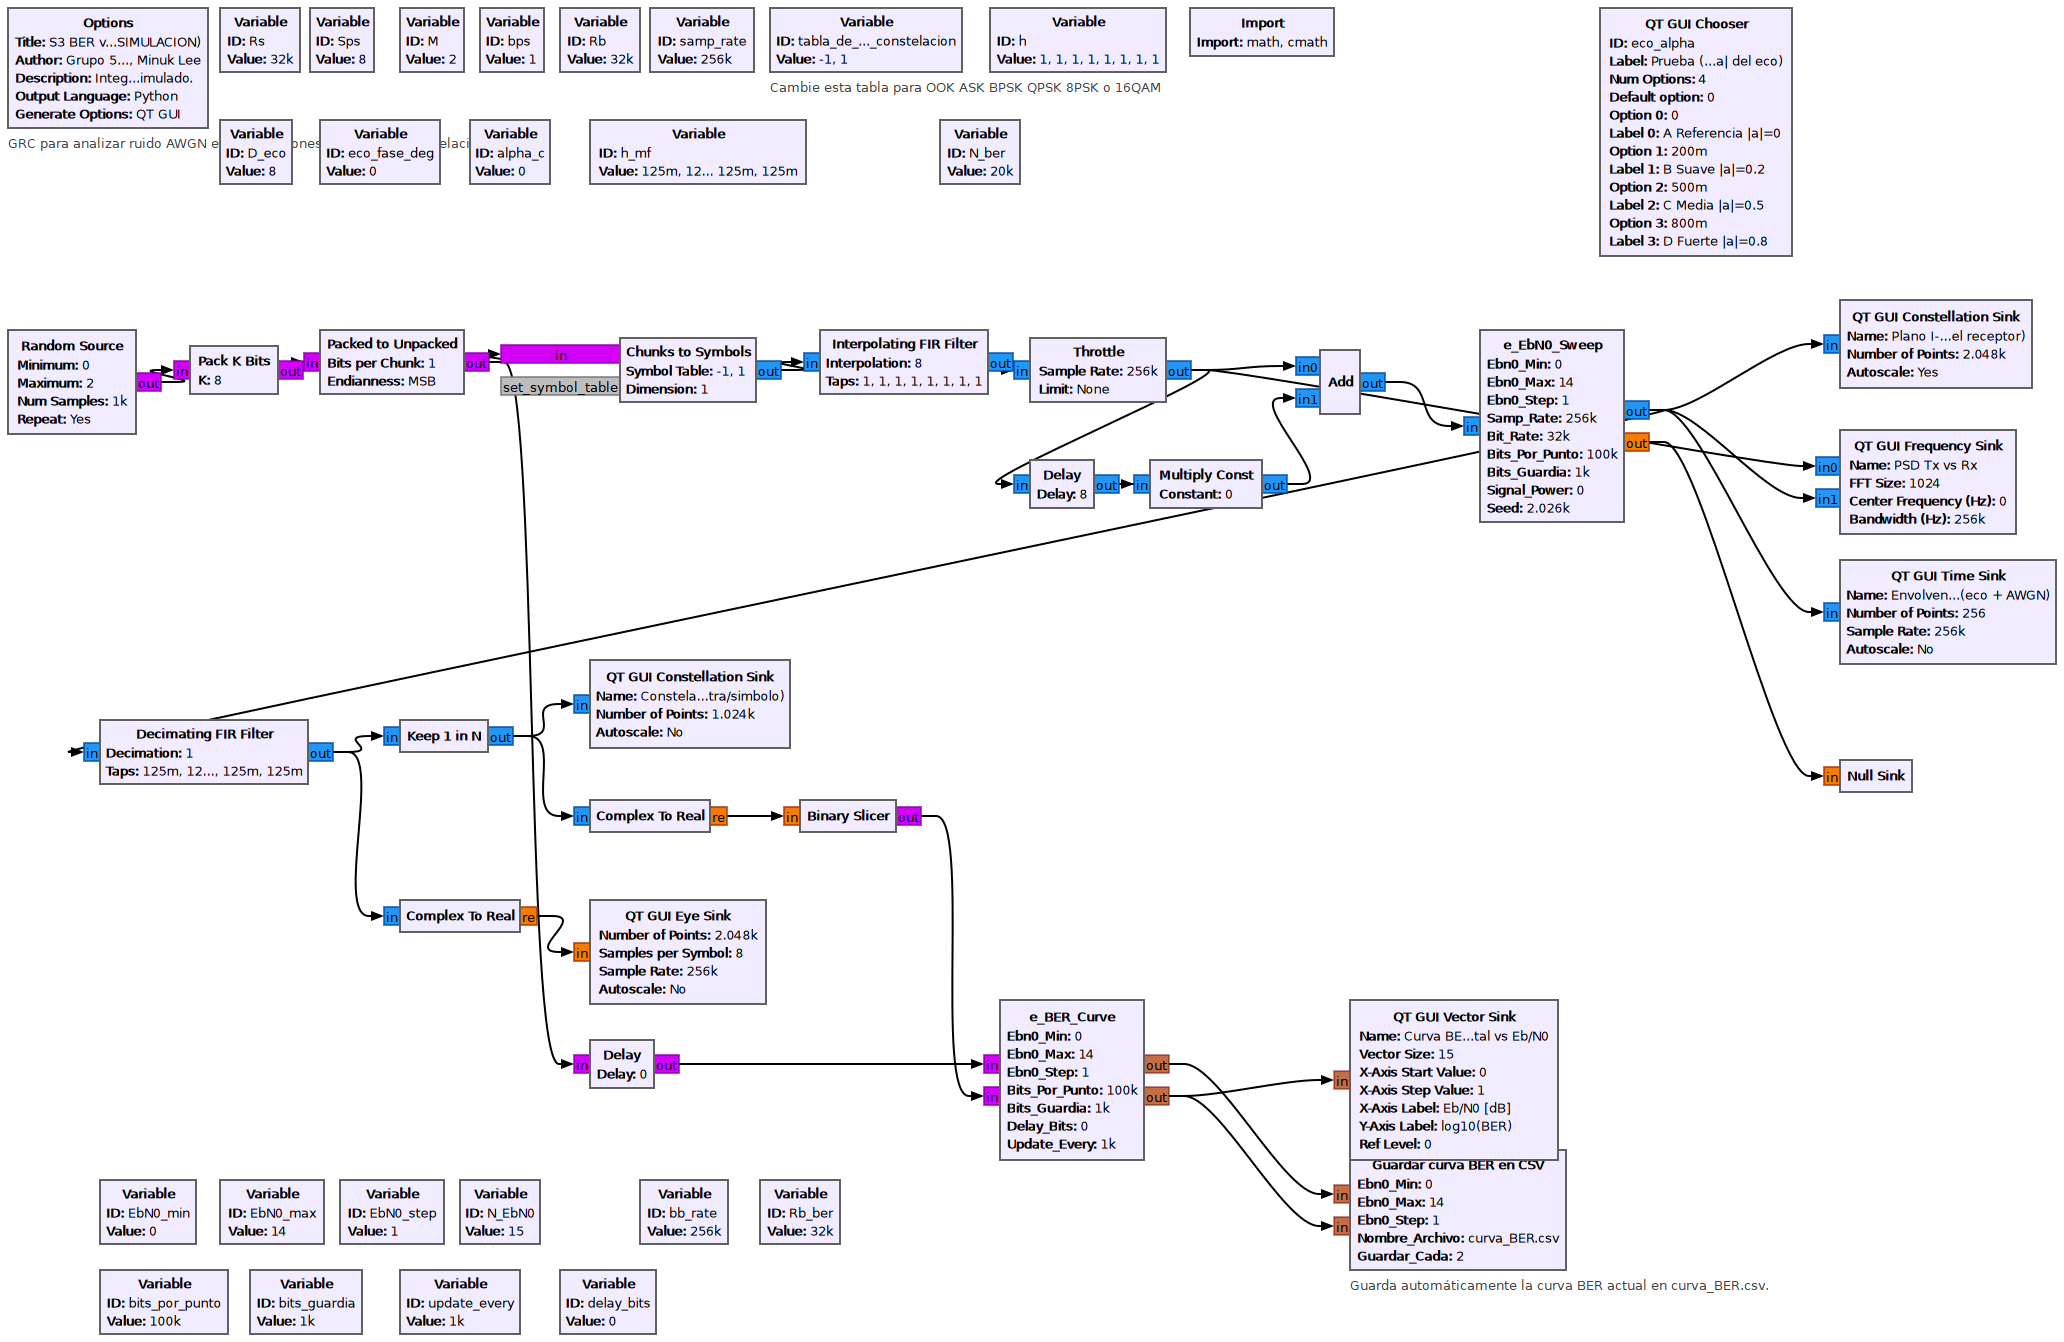
\includegraphics[width=\columnwidth]{GRC_S3_BER_Multitrayectoria_BPSK_Grupo5.png}
\caption{\texttt{S3\_BER\_Multitrayectoria\_BPSK\_Grupo5.grc}: \texttt{e\_EbN0\_Sweep} antes del receptor, y \texttt{e\_BER\_Curve} con la referencia Tx y los bits Rx.}
\label{fig:grc_ber}
\end{figure}

\section{Uso de herramientas de IA}
Se utilizó un asistente de IA (Claude, de Anthropic) para organizar el trabajo, generar los flujogramas a partir de los archivos del curso, automatizar la exportación de datos y las gráficas y proponer borradores de redacción. Todas las cifras provienen de ejecuciones de GNU Radio (3.10.9 en Linux y 3.10.12 en el equipo del grupo) y se contrastaron con la teoría. Las decisiones y conclusiones deben ser revisadas y asumidas por los integrantes del Grupo~5 antes de la entrega.

\begin{thebibliography}{10}

\bibitem{guia1} Escuela de Ingenierías Eléctrica, Electrónica y de Telecomunicaciones, ``Proyecto Integrador de Comunicaciones II: diseño, simulación y comunicación técnica de un sistema digital en GNU Radio -- Guía del estudiante,'' Universidad Industrial de Santander, Bucaramanga, Colombia, 2026.

\bibitem{guia2} O. Tíjaro y R. Zamora, ``Proyecto final de Comunicaciones II -- 27145. Fase 2: Modelado y simulación (Guía 2). Del transmisor conformado al diseño del receptor digital,'' Universidad Industrial de Santander, 2026.

\bibitem{guia3} O. Tíjaro y R. Zamora, ``Proyecto final de Comunicaciones II -- 27145. Fase 3: Implementación experimental en hardware SDR (Guía 3),'' Universidad Industrial de Santander, 2026.

\bibitem{guia4} O. Tíjaro y R. Zamora, ``Proyecto final de Comunicaciones II -- 27145. Fase 4: Validación final, ajuste y comparación experimental (Guía 4). Medición de desempeño mediante curvas BER vs.\ $E_b/N_0$,'' Universidad Industrial de Santander, 2026.

\bibitem{proakis2008} J. G. Proakis y M. Salehi, \emph{Digital Communications}, 5th ed. New York, NY, USA: McGraw-Hill, 2008.

\bibitem{rappaport2002} T. S. Rappaport, \emph{Wireless Communications: Principles and Practice}, 2nd ed. Upper Saddle River, NJ, USA: Prentice Hall, 2002.

\bibitem{saleh1987} A. A. M. Saleh y R. A. Valenzuela, ``A statistical model for indoor multipath propagation,'' \emph{IEEE J. Sel. Areas Commun.}, vol. 5, no. 2, pp. 128--137, Feb. 1987, doi: 10.1109/JSAC.1987.1146527.

\bibitem{hashemi1993} H. Hashemi, ``The indoor radio propagation channel,'' \emph{Proc. IEEE}, vol. 81, no. 7, pp. 943--968, Jul. 1993, doi: 10.1109/5.231342.

\bibitem{rappaport1989} T. S. Rappaport, ``Characterization of UHF multipath radio channels in factory buildings,'' \emph{IEEE Trans. Antennas Propag.}, vol. 37, no. 8, pp. 1058--1069, Aug. 1989.

\bibitem{gnuradio_symsync} GNU Radio Project, ``Symbol Sync,'' GNU Radio Wiki. [Online]. Available: \url{https://wiki.gnuradio.org/index.php/Symbol_Sync}

\end{thebibliography}

\end{document}
